\section{Введение.}

\clearpage

\section{Используемые технологии.}

При разработки данного ПО была использована микросервисная архитектура (\ref{d1}), которая в свою очередь
подразумевает использование архитектуры «клиент-сервер» (\ref{d2}).
\begin{definition}
    \label{d1}
    Микросервисная архитектура — вариант архитектуры программного обеспечения,
    ориентированный на взаимодействие насколько это возможно небольших, слабо связанных и легко изменяемых
    модулей — микросервисов.
\end{definition}
\begin{definition}
    \label{d2}
    Архитектура «клиент-сервер» — сетевая архитектура, в которой сетевая нагрузка распределена между поставщиками услуг,
    называемыми серверами, и заказчиками услуг, называемыми клиентами. Обычно клиенты и сервер расположены на разных
    машинах и взаимодействуют между собой через сеть посредством сетевых протоколов (\ref{d3}), однако они могут быть расположены
    и на одной машине.
\end{definition}
\begin{definition}
    \label{d3}
    Сетевой протокол — набор правил и очерёдности действий, позволяющий осуществлять соединение и
    обмен данными между двумя и более включёнными в сеть устройствами.
\end{definition}
В качестве серверной части используется ряд микросервисов, которые связаны с клиентской частью посредством
веб-сервера (\ref{d4}), а в качестве клиента используется веб-браузер (\ref{d5}).
\begin{definition}
    \label{d4}
    Веб-сервер — сервер, принимающий HTTP-запросы от клиентов, обычно веб-браузеров, и выдающий им HTTP-ответы,
    как правило, вместе с HTML-страницей, изображением, файлом, медиа-потоком или другими данными.
\end{definition}
\begin{definition}
    \label{d5}
    Веб-браузер — прикладное программное обеспечение для просмотра веб-страниц, компьютерных файлов и каталогов,
    управления веб-приложениями, а также для решения других задач.
\end{definition}
У такого решения существует ряд преимуществ:
\begin{enumerate}
    \item Существует множество реализаций веб-серверов для различных языков программирования.
    Это позволяет использовать уже готовые библиотеки и сосредоточиться непосредственно на написании функционала
    и реализации бизнес-логики.
    \item Использование веб-браузера в качестве клиента позволяет запускать приложение практически на любой платформе:
    десктопе, одноплатных компьютерах, мобильных устройствах, игровых консолях и пр.
    \item Т.к. все вычисления и логика работы выполняются на сервере, то снижаются требования к устройствам, на которых
    запущена клиентская часть приложения.
\end{enumerate}
Данные между клиентом и сервером, а также между отдельными микросервисами передаются в JSON формате (\ref{d6}). Компоненты
серверной части общаются между собой по протоколу MQTT (\ref{d7}).
\begin{definition}
    \label{d6}
    JSON — текстовый формат обмена данными, основанный на подмножестве языка JavaScript.
\end{definition}
\begin{definition}
    \label{d7}
    MQTT — упрощённый сетевой протокол, работающий поверх TCP/IP, ориентированный для обмена сообщениями между устройствами
    по принципу издатель-подписчик. 
\end{definition}
Т.к. клиентская часть реализованна в виде веб-приложения, то для её написания использовался язык программирования
JavaScript (\ref{d10}), язык разметки HTML (\ref{d8}) и язык стилей CSS (\ref{d9}).
\begin{definition}
    \label{d8}
    HTML — cтандартизированный язык разметки документов в сети Интернет.
    Язык HTML интерпретируется браузерами. Полученный в результате интерпретации форматированный текст
    отображается на экране монитора компьютера или мобильного устройства.
\end{definition}
\begin{definition}
    \label{d9}
    CSS — формальный язык описания внешнего вида документа, написанного с использованием языка разметки.
\end{definition}
\begin{definition}
    \label{d10}
    JavaScript — мультипарадигменный язык программирования. Поддерживает объектно-ориентированный, императивный и
    функциональный стили. Наиболее широкое применение находит в браузерах как язык сценариев для придания интерактивности
    веб-страницам.
\end{definition}
Основной функционал серверной части приложения написан на языке Python (\ref{d11}). Однако для написания файлов конфигураций
использовались и другие языки, например XML (\ref{d12}) и YAML (\ref{d13}).
\begin{definition}
    \label{d11}
    Python — высокоуровневый язык программирования общего назначения, ориентированный на повышение производительности
    разработчика и читаемости кода.
\end{definition}
\begin{definition}
    \label{d12}
    XML — расширяемый язык разметки. XML разрабатывался как язык с простым формальным синтаксисом, удобный для создания
    и обработки документов программами и одновременно удобный для чтения и создания документов человеком.
    Язык называется расширяемым, поскольку он не фиксирует разметку, используемую в документах:
    разработчик волен создать разметку в соответствии с потребностями к конкретной области, будучи ограниченным лишь
    синтаксическими правилами языка.
\end{definition}
\begin{definition}
    \label{d13}
    YAML — формат сериализации данных, концептуально близкий к языкам разметки, но ориентированный на удобство
    ввода-вывода типичных структур данных многих языков программирования.
\end{definition}
Для обеспечения одновременной работы сразу со множеством клиентов серверная часть использует несколько видов конкурентности
(\textit{concurrency}): потоки (\textit{threads}) (\ref{d14}) и асинхронный ввод/вывод (\ref{d15}).
\begin{definition}
    \label{d14}
    Поток выполнения — наименьшая единица обработки, исполнение которой может быть назначено ядром операционной системы.
    Реализация потоков выполнения и процессов в разных операционных системах отличается друг от друга, но в большинстве
    случаев поток выполнения находится внутри процесса. Несколько потоков выполнения могут существовать в рамках одного
    и того же процесса и совместно использовать ресурсы, такие как память, тогда как процессы не разделяют этих ресурсов.
\end{definition}
\begin{definition}
    \label{d15}
    Асинхронный ввод/вывод — форма неблокирующей обработки ввода/вывода, которая позволяет процессу
    продолжить выполнение не дожидаясь окончания передачи данных.
\end{definition}
Микросервисы в серверной части приложения используют технологии виртуализации (\ref{d16}) и контейнеризации (\ref{d17}).
Для автоматического развёртывания и удобства управления контейнерами используется ПО Docker (\ref{d18}).
\begin{definition}
    \label{d16}
    Виртуализация — предоставление набора вычислительных ресурсов, абстрагированное от аппаратной реализации,
    и обеспечивающее при этом логическую изоляцию друг от друга вычислительных процессов, выполняемых на одном
    физическом ресурсе. 
\end{definition}
\begin{definition}
    \label{d17}
    Контейнеризация — метод виртуализации, при котором ядро операционной системы поддерживает несколько изолированных
    экземпляров пространства пользователя вместо одного. Эти экземпляры (обычно называемые контейнерами) с точки зрения
    пользователя полностью идентичны отдельному экземпляру операционной системы.
\end{definition}
\begin{definition}
    \label{d18}
    Docker — программное обеспечение для автоматизации развёртывания и управления приложениями в средах с
    поддержкой контейнеризации. Позволяет «упаковать» приложение со всем его окружением и зависимостями в контейнер,
    а также предоставляет среду по управлению контейнерами.
\end{definition}

\clearpage

\section{Архитектура системы.}

Как было сказано ранее данное ПО использует микросервисную архитектуру (\ref{d1}). Каждый компонент системы предоставляет
собой модуль, который работает в Docker-контейнере (\ref{d18}) и взаимодействует с другими модулями по сети.
Схема взаимодействия представлена на рис. \ref{fig:arch}.

\begin{figure}[h]
    \centering
    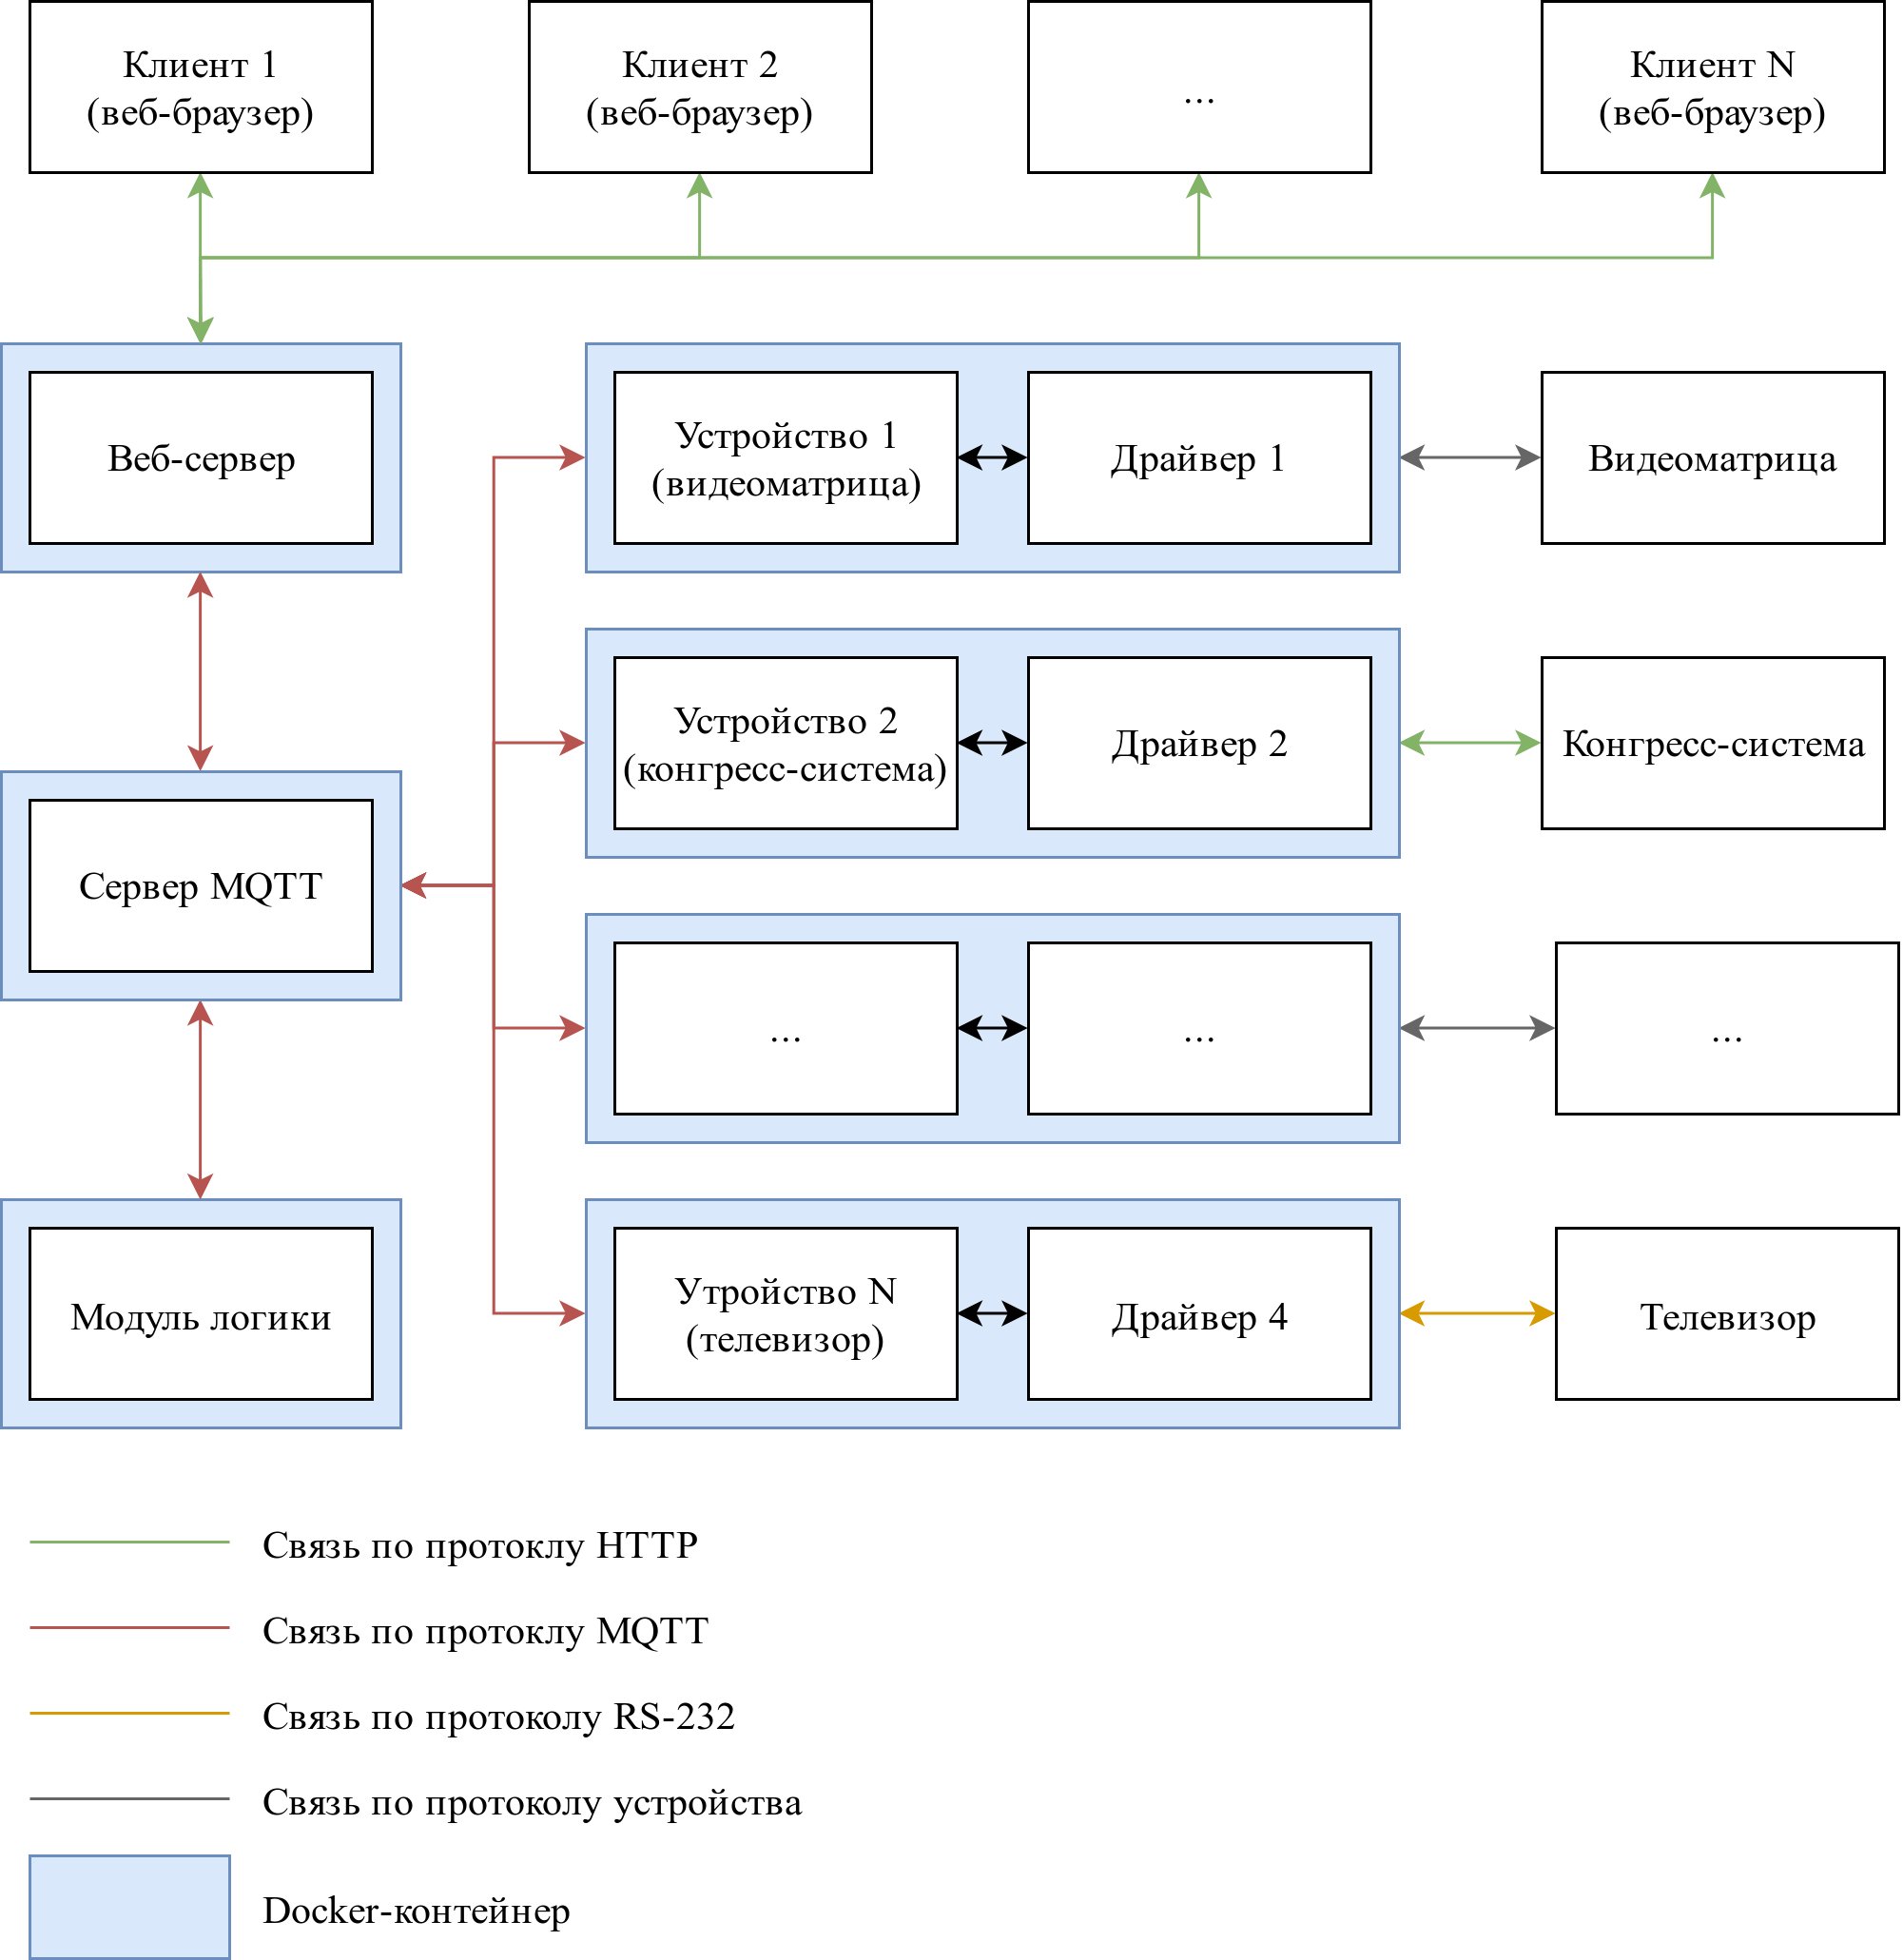
\includegraphics[width=1\linewidth]{arch.png}
    \caption{Схема взаимодействия компонентов системы.}
    \label{fig:arch}
\end{figure}

\noindent Благодаря тому, что компоненты программы общаются друг с другом по сети, приложение может быть запущено как
на одной машине, так и на нескольких (вплоть до того, что каждый Docker-контейнер может быть запущен на отдельном сервере).
Такая распределённая система даёт следующие преимущества:
\begin{enumerate}
    \item \textbf{Производительность и масштабируемость}. При необходимости можно перераспределить нагрузку на сервер
    просто перенеся некоторые из Docker-контейнеров на другой, более мощный компьютер.
    \item \textbf{Отказоустойчивость} - система сохранит частичную или полную работоспособность в случае отказа одного
    или нескольких компонентов.
\end{enumerate}

\subsection{Основные компоненты системы.}

Первое, что видит пользователь приложения это интерфейс (рис. \ref{fig:main_screen}). Для его отрисовки браузер запрашивает
у сервера те элементы, которые должны присутствовать на экране. Для удобства разработки был написан собственный механизм
создания таких интерфейсов, работающий следующим образом. Любой объект на экране состоит из множества простых элементов.
Простые элементы бывают 5 видов: \textit{группа}, \textit{надпись}, \textit{картинка}, \textit{поле для ввода} и
\textit{слайдер}. Комбинируя их в любом количестве мы можем создавать объекты любой сложности. Например, объединив
\textit{надпись} и \textit{группу} можно сделать кнопку с текстом, а если добавить в эту \textit{группу} \textit{картинку},
то будет кнопка с текстом и иконкой.

\begin{figure}[h]
    \centering
    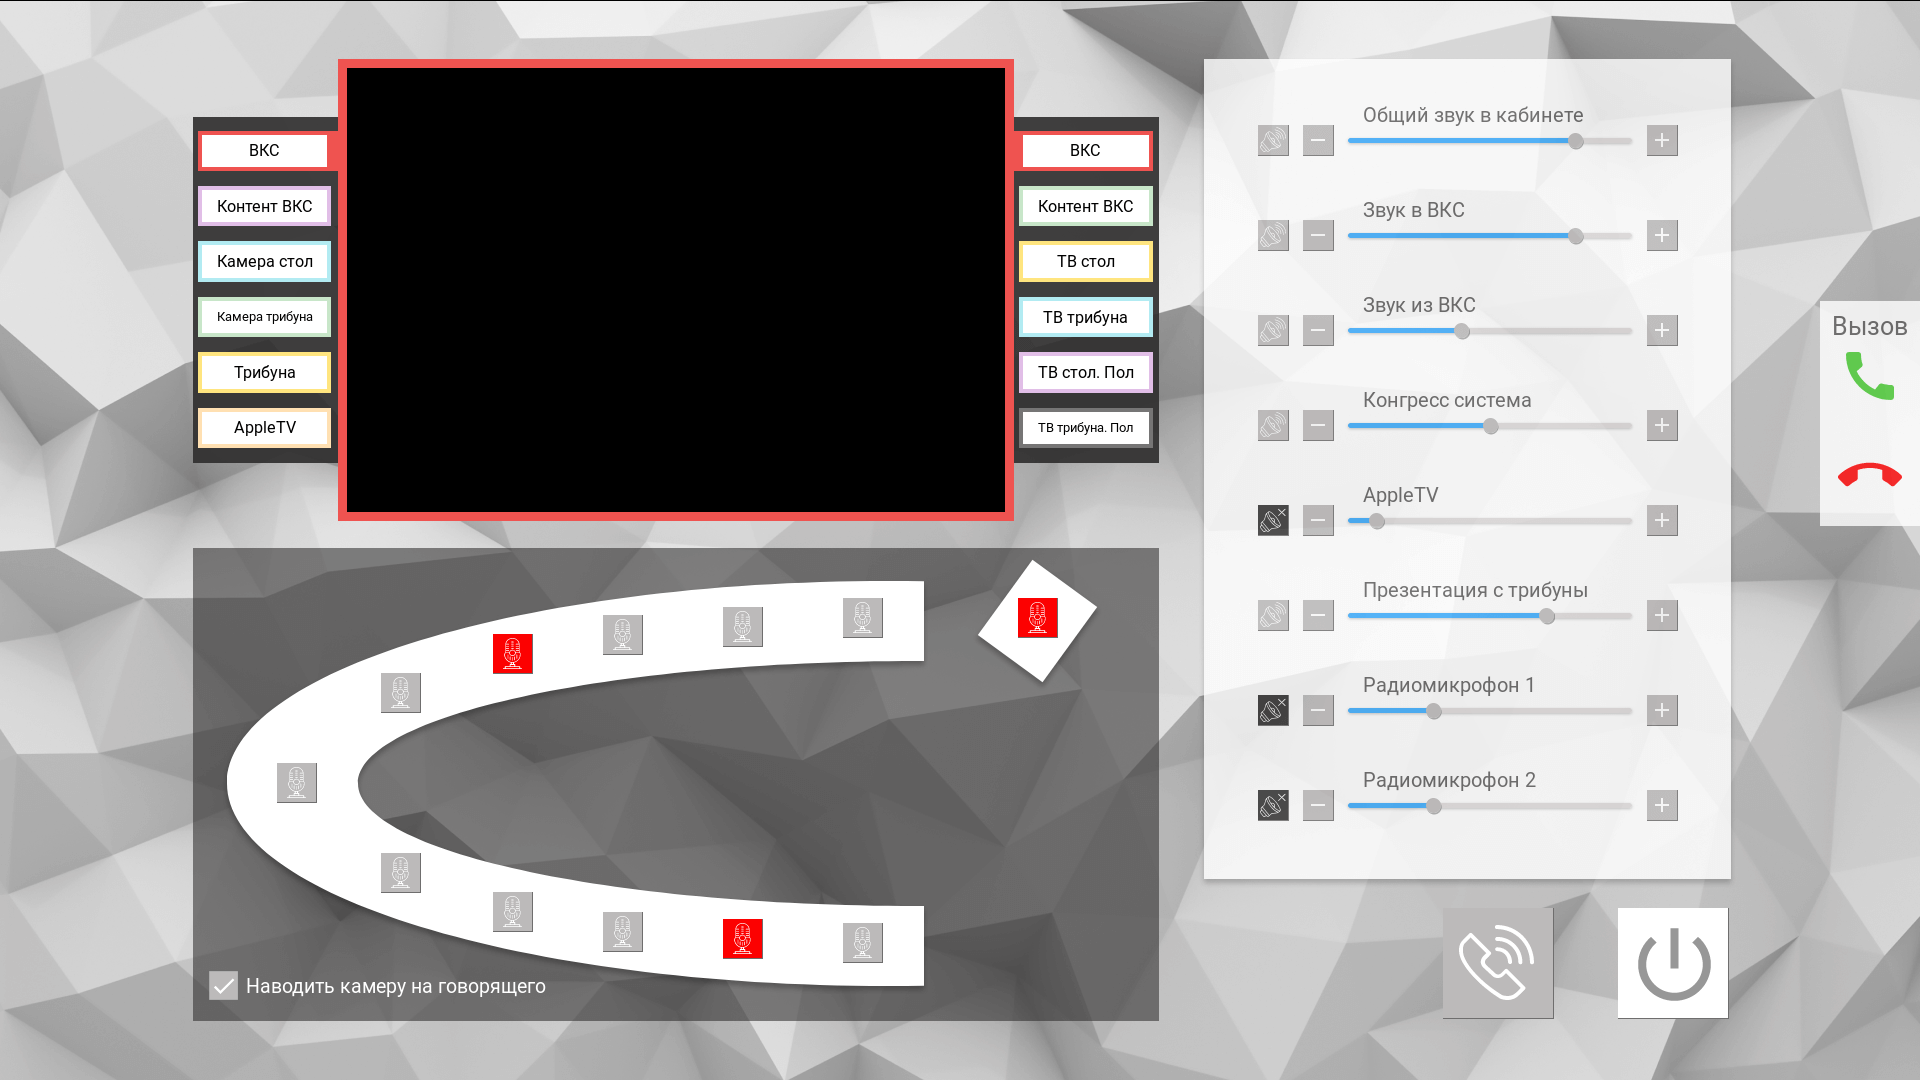
\includegraphics[width=1\linewidth]{main_screen.png}
    \caption{Главный экран приложения.}
    \label{fig:main_screen}
\end{figure}

\noindent Вся разметка страницы хранится в формате JSON (\ref{d6}). После того, как браузер получил данные от сервера он
преобразует эти данные в HTML (\ref{d8}) для отображения на странице. Этот подход отличается от более стандартного:
веб-сервер отдаёт браузеру готовый HTML код и браузер сразу рендерит страницу. Данный способ работы был выбран из-за того,
что он позволяет создать визуальный редактор интерфейса, который будет работать прямо в браузере. В случае же с
преобразованием JSON в HTML на сервере это привело бы к написанию кода с одинаковой функциональностью в 2-х различных
местах программы.

~\

% Взаимодействие с клиентами происходит через веб-сервер (\ref{d4}). Для его написанния используется язык Python (\ref{d11}),
% а также фреймворк \textit{aiohttp}, который работает с помощью библиотеки для асинхронных вызовов \textit{asyncio}.

\subsection{Взаимодействие компонентов.}

Общаясь между собой компоненты системы передают информацию в формате JSON (\ref{d6}) по следующему протоколу:
\lstinputlisting[caption=Структура запроса.]{request.json}
\lstinputlisting[caption=Структура ответа.]{response.json}
Значения полей:
\begin{enumerate}
    \item \textit{SENDER\_NAME} - адрес отправителя конкретного запроса или ответа.
    \item \textit{INITIATOR\_NAME} - адрес отправителя первого запроса из этой цепочки (с кого началась обработка события).
    \item \textit{PRIORITY\_LEVEL} - приоритет запроса.
    \item \textit{COMMAND\_ID} - уникальный идентификатор запроса. Повторяется в ответе.
    Используется для привязки ответов, получаемых асинхронно.
    \item \textit{COMMAND\_NAME} - команда.
    \item \textit{EVENT\_NAME} - событие.
    \item \textit{PARAMETERS} - параметры команды или события в формате «ключ-значение».
    \item \textit{DESCRIPTION} - человекочитаемое описание события или ошибки.
    \item \textit{STATUS} - результат выполнения команды.
\end{enumerate}
